\section{Anhang}
\subsection{Testergebnisse}

\subsection{Abmessungen}

\subsection{Datenblattauszüge}

\textcolor{blue}{Im Anhang befinden sich weitere Detailinformationen des Projekts wie\\
•	Datenblattauszüge, Fertigungsunterlagen (PCB-Layouts, Gehäusezeichnungen, 3D-Druckunterlagen, Montageanleitungen,…) etc.\\
•	sämtliche geforderten Projektmanagementdokumente\\
•	ein Businessplan (optional)
}

\subsection{Projektmanagement}
\textcolor{blue}{In diesem Kapitel soll auf das Projektmanagement des Projektes eingegangen werden. Zu Beginn empfiehlt es sich, die einzelnen Bereiche des Projektmanagements zu erklären und anschließend in einzelnen Kapiteln zu behandeln.}

\subsubsection{Aufgabenstellung des Gesamtprojekts}
\textcolor{blue}{Fügen Sie an dieser Stelle den Text der genehmigten Aufgabenstellung ein, der in die Diplomarbeitsdatenbank  eingegeben wurde.}

\subsubsection{Scrum-Projektplan}
\textcolor{blue}{Fügen Sie hier den vollständigen Scrum-Projektplan, wobei die Nummern der Tasks mit der Arbeitszeitaufzeichnung übereinstimmen müssen. Der Scrum-Projektplan kann auf mehrere Seiten aufgeteilt werden.}

\bgroup
    \centering
    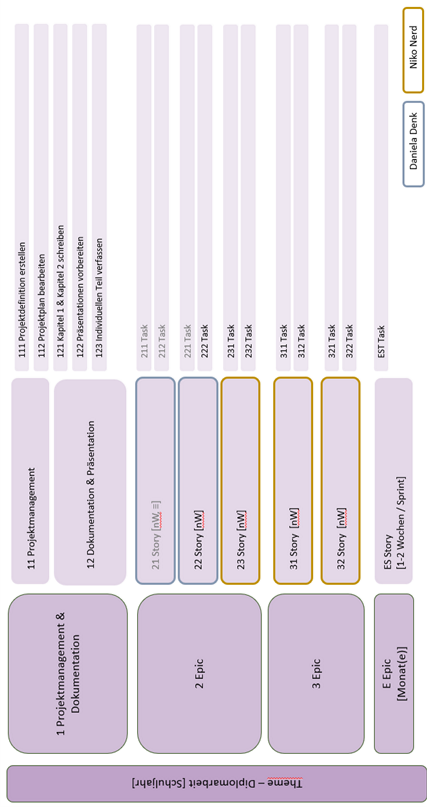
\includegraphics[width=0.6\textwidth]{Scrum_Projektplan_mit_Tasks.png}
    \captionof{figure}{Scrum Projektplan mit Tasks}
\egroup

\newpage
\subsubsection{Terminplanung}

\newpage
\subsection{Inbetriebnahme}
\color{blue}
Nachdem typische Projekte aus mehreren Komponenten bestehen, ist es oft nicht trivial die einzelnen Komponenten korrekt zu konfigurieren und das Gesamtsystem in Betrieb zu nehmen. In diesem Kapitel soll eine vollständige, präzise und trotzdem möglichst kompak-te Anleitung zur Inbetriebnahme des Systems dargelegt werden. Die Schritte sollen in dem Detailgrad beschrieben werden, dass ein durchschnittlicher Schüler des vierten Jahrganges das Projekt in Betrieb nehmen kann. Exemplarisch sollten Punkte wie die folgenden be-handelt werden – die Aufzählung ist nicht vollständig):
\begin{itemize}
    \item Treiberinstallationen und Systemkonfigurationen
    \item Zu empfehlen wäre bei Server-Installationen ein Setup-Script, welches auf einem vordefinierten Docker-container aufbaut.
    \item Welche Schritte sind notwendig, um das Projekt mit dem vorhandenen Code / Schaltplänen (auf GIT, CD, Netzlaufwerk, etc.) in Betrieb zu nehmen.
    \item Bei Schaltungen mit mehreren Platinen muss beschrieben werden, wie diese mit-einander verbunden werden müssen.
\end{itemize}
\color{black}

\newpage
\subsection{Kostenaufstellung}
\textcolor{blue}{Für die Kalkulation im Gesamtprojekt sind folgende Kosten zu erfassen: \\
•	Kosten für Material (Hard- und Software)\\
•	externe Kosten (z.B.: Zukauf von Sensoren, Funkmodule, spezielle Entwicklungsum-gebungen, etc.) 
}
\begin{figure}[h]
    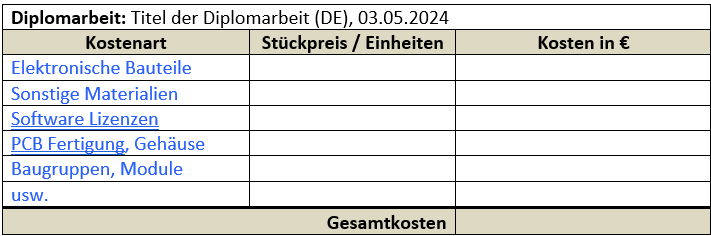
\includegraphics[width=0.8\textwidth]{Kostenaufstellung.png}
    \centering
    \caption{Kostenaufstellung}
\end{figure}

\newpage
\subsection{Besprechungsprotokolle}
\textcolor{blue}{Eine entsprechende Vorlage wird auf den Schulrechner in Form einer Word-Vorlage be-reitgestellt. Scannen Sie die vier Besprechungsprotokolle (laut Vorlage) ein und fügen Sie diese nachfolgend an (eine A4-Seite pro Protokoll)\\
Protokolle zu den einzelnen Iterationen:\\
•	Vorprojektphase\\
•	Iteration 1\\
•	Iteration 3\\
•	Iteration 5\\
Die Termine und Inhalte/Projektstatus entsprechen denen der Iterationspräsentationen.
}

\newpage
\subsection{Arbeitsnachweis}
\textcolor{blue}{Jedes Teammitglied (Schüler/in) hat einen vollständigen Arbeitszeitnachweis, der außer-halb des Unterrichts verrichteten Tätigkeiten, in tabellarischer Form zu erbringen. \\Eine entsprechende Vorlage wird auf den Schulrechner in Form einer Excel-Vorlage bereitgestellt.}

\newpage
